\block{3. Temporal Analysis}{%
    \noindent%
    \begin{minipage}[t]{0.48\linewidth}%
        \centering
        {\small\textbf{Intra-party Cohesion Over Time}}\\[0.3cm]
        
\includegraphics[width=0.95\linewidth]{fig5_cohesion.png}\\[0.3cm]
        \flushleft
        \begin{itemize}
            \item \textbf{Coalition Discipline:} KO, PSL-TD, Lewica stay above 95\% throughout the term.
            \item \textbf{Konfederacja KP Split (2024):} Cohesion collapsed — the sharpest internal crisis in the dataset.
            \item \textbf{Presidential Effect:} Cohesion dips across all parties during election rounds (May--Jun 2025).
        \end{itemize}
    \end{minipage}%
    \hfill%
    \begin{minipage}[t]{0.48\linewidth}%
        \centering
        {\small\textbf{Club Attendance Over Time}}\\[0.3cm]
        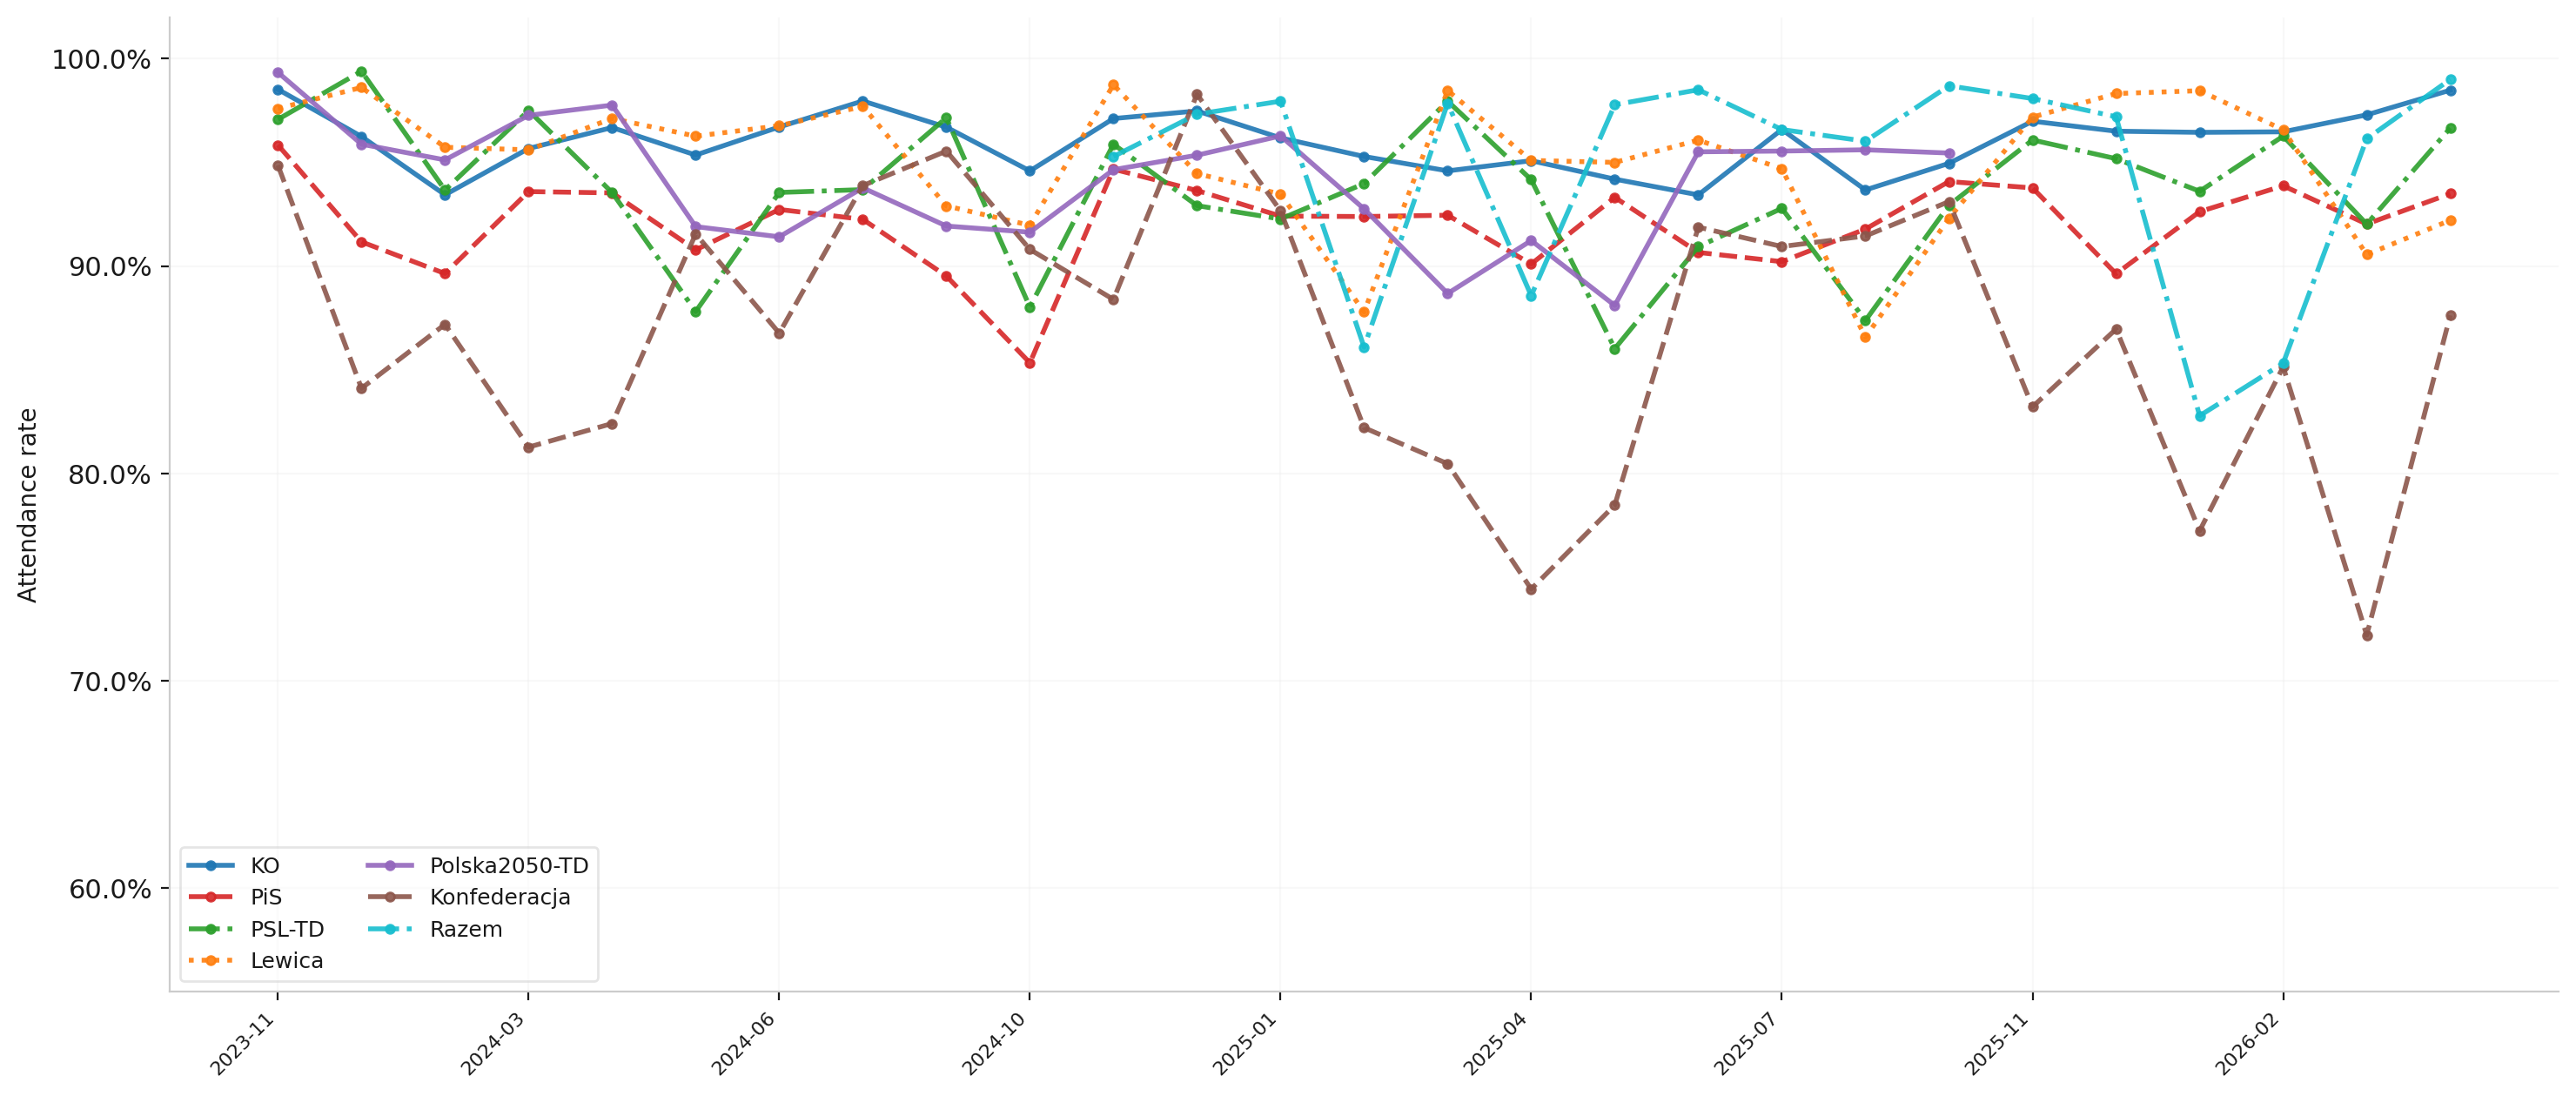
\includegraphics[width=0.95\linewidth]{fig12_attendance_over_time.png}\\[0.3cm]
        \flushleft
        \begin{itemize}
            \item \textbf{PiS Drops:} Opposition parties show the most volatile attendance — dips below 75\%.
            \item \textbf{Coalition Consistency:} Coalition clubs generally maintain attendance above 90\%.
            \item \textbf{Konfederacja:} Sharpest and most frequent attendance drops — correlating with contested legislative sessions where their vote would be decisive.
        \end{itemize}
    \end{minipage}%
}
